% Created 2026-09-23 Wed 12:38
% Intended LaTeX compiler: pdflatex
\documentclass[fleqn]{article}
\usepackage[utf8]{inputenc}
\usepackage[T1]{fontenc}
\usepackage{graphicx}
\usepackage{longtable}
\usepackage{wrapfig}
\usepackage{rotating}
\usepackage[normalem]{ulem}
\usepackage{amsmath}
\usepackage{amssymb}
\usepackage{capt-of}
\usepackage{hyperref}
\usepackage{amsmath}
\usepackage{mathtools}
\usepackage{braket}
\usepackage{tikz}
\usepackage{tikz-cd}
\usepackage{parskip}
\usepackage{enumitem}
\usepackage[
letterpaper,
top=2cm,
bottom=2cm,
left=3cm,
right=3cm,
marginparwidth=1.75cm
]{geometry}
\setlist[itemize]{label=--}
\date{\today}
\title{}
\hypersetup{
 pdfauthor={},
 pdftitle={},
 pdfkeywords={},
 pdfsubject={},
 pdfcreator={Emacs 30.2 (Org mode 9.7.11)}, 
 pdflang={English}}
\begin{document}

\tableofcontents

\section{People}
\label{sec:org57ad1c2}

Avionics:
\begin{itemize}
\item Nick (also propulsion)
\end{itemize}

Payload:
\begin{itemize}
\item Mica (contact about Pilotix)
\end{itemize}

Propulsion:
\begin{itemize}
\item Francesco (adapters)
\item Robert (parametric)
\item Nils (WhatsApp guy, propulsion not-lead)
\item David (not-fuel grain guy)
\end{itemize}

Airbreak:
\begin{itemize}
\item Iheb Bouakira (CFD)
\end{itemize}

Python RocketCEA
\section{Code}
\label{sec:orgfc6e234}

Input variables:

\begin{itemize}
\item Tank
\begin{itemize}
\item Injector hole count
\item Injector total hole area
\end{itemize}

\item Fuel grain:
\begin{itemize}
\item Fuel inner radius
\item Fuel outer radius
\end{itemize}

\item Combustion chamber and nozzle:
\begin{itemize}
\item Throat length
\item Throat radius
\item Converging throat section angle
\item Nozzle length
\item Inner liner thickness
\item Pre-combustion chamber length
\item Post-combustion chamber length
\item Chamber inner radius
\item Chamber outer radius
\end{itemize}
(I want to specify all of these in a generic manner as \(f(z)\))

\item Thrust
\item Burn time
\end{itemize}

Output variables:
\begin{itemize}
\item Specific impulse
\end{itemize}

\begin{figure}[htbp]
\centering
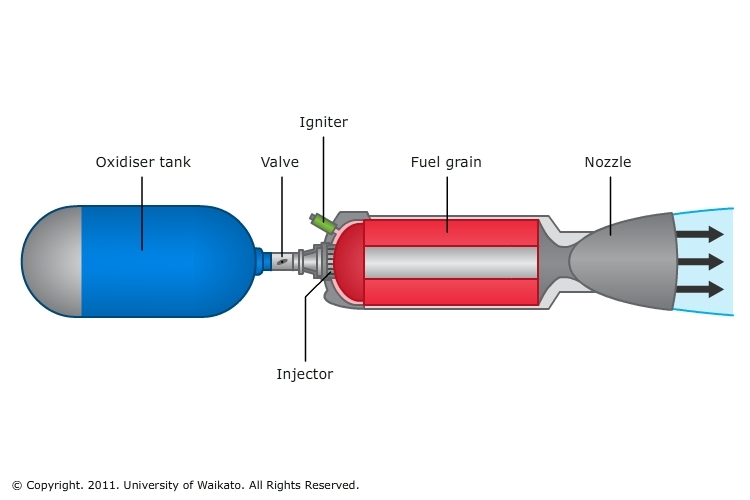
\includegraphics[width=.9\linewidth]{./fig/Hybrid-rocket-engine.jpg}
\caption{\label{fig:org956471d}Design of a hybrid rocket engine}
\end{figure}

\begin{figure}[htbp]
\centering
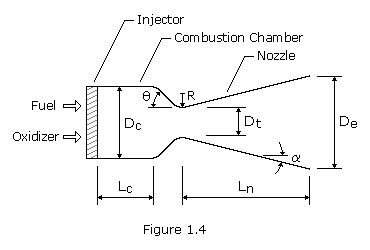
\includegraphics[width=.9\linewidth]{./fig/convergent-divergent-nozzle.png}
\caption{\label{fig:org669a29e}Design of a convergent-divergent nozzle}
\end{figure}
\subsection{Theory}
\label{sec:orge2420d2}

\subsubsection{Notation}
\label{sec:org2a09a7d}

\begin{description}
\item[{\(h\)}] altitude above sea level

\item[{\(\mathcal A\)}] attitude, represented by either a 3-vector of Eulerian angles
or a quaternion

\item[{\((\cdot)^*, (\cdot)_\text{t}\)}] value of a variable at the throat of the
convergent-divergent nozzle

\item[{\((\cdot)_\text{c}\)}] value of a variable inside the combustion chamber at the
entrance of the nozzle

\item[{\((\cdot)_\text{e}\)}] value of a variable at the exit of the nozzle

\item[{\((\cdot)_\text{amb}\)}] "ambient" value of a variable in the environment
outside the rocket, for example \(P_\text{amb}\)
\end{description}
\subsubsection{General}
\label{sec:org29d9853}

Ballpark of the total rocket structural mass: \textasciitilde{}60 kg

2D attitude lookup table:
\(\mathcal A : \mathbb R^3, \mathbb R^3 \to \mathbb R^3 | \mathbb H\),
\(\mathcal A(\mathbf x, \mathbf v)\)

Ideal rocket equation:

\begin{equation*}
\Delta v
= v_e \ln\frac{m_\text{i}}{m_\text{f}}
= I_\text{sp} g_0 \ln\frac{m_\text{i}}{m_\text{f}}
\end{equation*}

Thrust equations:

\begin{equation*}
\dot{m} = \rho_\text{e} u_\text{e} A_\text{e}
\end{equation*}

\begin{equation*}
T
= \dot{m} u_\text{e} + (P_\text{e} - P_\text{a}) A_\text{e}
= \dot{m} u_\text{e} + P_\text{e} A_\text{e} - P_\text{a} A_\text{e}
= T_\text{vac} - (P_\text{a} \cdot A_\text{e})
\end{equation*}

Total force acting on the rocket:

\begin{equation*}
F = T - D
\end{equation*}

(thrust - drag)

References:

\url{https://www.grc.nasa.gov/WWW/k-12/airplane/rktthsum.html}

\url{https://rrs.org/2023/01/28/making-correct-parabolic-nozzles/}
\subsubsection{Nonlinearity}
\label{sec:orgc95f9d5}

In OpenMDAO, each component maps its inputs to its outputs, \(y = f(x)\). When
components connect in a chain, OpenMDAO simply evaluates them
sequentially. Components taken together in a group form a system of equations
with the internal equations of their components.

In the \texttt{PropulsionGroup} component group, the components form a closed loop, and
the system of equations happens to be non-linear. Explicitly, it consists of the
following:

\begin{enumerate}
\item Injector flow (Bernoulli orifice)

\begin{equation*}
\dot{m}_\text{ox}
= C_\text{d} A_\text{inj}
  \sqrt{2\rho_\text{ox} (P_\text{tank} - P_\text{c})}
\end{equation*}

\item Chamber chemistry (Gibbs free energy equilibrium)

\begin{equation*}
c^* = f_\text{CEA} (P_\text{c}, \mathrm{MR})
\end{equation*}

\item Nozzle choking (1D isentropic throat flow)

\begin{equation*}
P_\text{c}
= \frac{\dot{m}_\text{prop} \cdot c^*}{A_\text{t}}
= \frac{\dot{m}_\text{ox} \left(1 - \frac{1}{\mathrm{MR}}\right)c^*}
       {A_\text{t}}
\end{equation*}
\end{enumerate}

Substituting (1) and (2) into (3) we obtain the following master equation:

\begin{equation*}
P_\text{c}
= \left[
    \frac{C_\mathrm{d} A_\text{inj} \left(1 + \frac{1}{\mathrm{MR}}\right)}
         {A_\text{t}}
  \right]
  \cdot \sqrt{2\rho_\text{ox} (P_\text{tank} - P_\text{c})}
  \cdot c^* (P_\text{c}, \mathrm{MR})
\end{equation*}

This system is nonlinear and cannot be solved in closed form for three reasons:

\begin{enumerate}
\item The pressure drop \(\Delta P = P_\text{tnk} - P_\text{c}\) sits inside a square
root

\item \(c^* (P_\text{c}, \mathrm{MR})\) is not constant, high pressure would suppress
molecular dissociation, which changes gas molecular weight and temperature
nonlinearly

\item Chamber pressure \(P_\text{c}\) appears both under the square root and inside
the CEA chemistry table, creating an implicit self-dependency
\end{enumerate}

To solve this, define the \emph{residual function} \(R(P_\text{c}) = 0\):

\begin{equation*}
R(P_\text{c})
= P_\text{c}
  - \left[
    \frac{C_\mathrm{d} A_\text{inj} \left(1 + \frac{1}{\mathrm{MR}}\right)}
         {A_\text{t}}
  \right]
  \cdot \sqrt{2\rho_\text{ox} (P_\text{tank} - P_\text{c})}
  \cdot c^* (P_\text{c}, \mathrm{MR})
= 0
\end{equation*}

OpenMDAO's \texttt{NewtonSolver} solves \(R(P_\text{c})=0\) using an initial guess and
tangent lines:

\begin{equation*}
P_\text{c}^{(k+1)}
= P_\text{c}^{(k)}
  - \frac{R(P_\text{c}^{(k)})}{\mathrm{d} R / \mathrm{d} P_\text{c}}
\end{equation*}
\subsubsection{Tank}
\label{sec:orge6a3db4}

\sout{60} 70 bar tank pressure

Should be roughly 30-40 kg
\subsubsection{Plumbing/injector}
\label{sec:orgcdd15f1}

\textasciitilde{}30 bar pressure loss between tank and fuel grain

Either pressure drop or mass flow rate across the injector
\subsubsection{Chamber/nozzle}
\label{sec:orgb490a9a}

In the following, let the asterisk superscript denote the value of a function of
the vertical position \(z\) at the throat.

Area-mach relation:

\begin{equation*}
\frac{A(z)}{A^*}
= \frac{1}{M(z)} \left[
  \frac{2}{\gamma+1} \left(1 + \frac{\gamma-1}{2} M^2(z)\right)
\right]^{\frac12\frac{\gamma+1}{\gamma-1}}
\end{equation*}

where \(A^*\) is the throat area, \(M(z)\) is the Mach number at coordinate \(z\).

Mass flow rate:

\begin{equation*}
\dot{m}
= A(z) P(z) \sqrt{\frac{\gamma}{T R}} M(z) \left[
  1 + \frac{\gamma-1}{2}M^2(z)
\right]^{-\frac12 \frac{\gamma+1}{\gamma-1}}
\end{equation*}

where \(T\) is the chamber temperature, \(R\) is the ideal gas constant, \(\gamma\)
the specific heat ratio. For maximum flow rate, set \(M(z^*)=1\):

\begin{equation*}
\dot{m}
= A^* P^* \sqrt{\frac{\gamma}{TR}}
  \left[ \frac{\gamma+1}{2} \right]^{-\frac12 \frac{\gamma+1}{\gamma-1}}
\end{equation*}

This is then used to calculate thrust according to the previous formula

References:

\url{https://web.stanford.edu/\~cantwell/AA284A\_Course\_Material/Karabeyoglu\%20AA\%20284A\%20Lectures/AA284a\_Lecture2.pdf}

\url{https://www.grc.nasa.gov/WWW/K-12/airplane/astar.html}

\url{https://www.grc.nasa.gov/WWW/K-12/airplane/isentrop.html}

\url{https://rrs.org/2023/01/28/making-correct-parabolic-nozzles/}
\subsection{The CEA rocket solver}
\label{sec:org5183db0}

The CEA rocket solver is a thermodynamic state-finder that follows a parcel of
gas as it moves from the chamber to the exit assuming an isentropic path (line
of constant entropy). The solver always calculates at least two points: the
chamber and the throat. All points specified in the parameters by the user will
then be appended to the list of snapshot points.

Consider packaging the incoming reactant mixture as follows:

\begin{verbatim}
mixture = [
    { name: "H2(L)", temp: 20.27, fraction: 1.0, fuel_weight: 1.0, oxidant_weight: 0.0 },
    { name: "O2(L)", temp: 90.17, fraction: 1.0, fuel_weight: 0.0, oxidant_weight: 0.1 },
]
\end{verbatim}

Isolating the essential arguments of the CEA rocket solver, one can define a
function of the following form:

\begin{verbatim}
def solve(
    mixture : dict,        # mixture component dictionary
    pc      : float,       # chamber pressure
    subar   : list[float], # subsonic area ratio
    supar   : list[float]  # supersonic area ratio
) -> cea.RocketSolution:

    ... # implementation details

    solver.solve(solution, weights, pc, pi_p, subar=subar, supar=supar, hc)

    return solution
\end{verbatim}

\begin{description}
\item[{\texttt{mixture}}] is some kind of table packaging together the chemical components
of the fuel and oxidizer, their temperatures

\item[{\texttt{pc}}] being the chamber pressure, a design variable

\item[{\texttt{subar}}] being the subsonic area ratio, \(A_\text{c}/A^*\)

\item[{\texttt{supar}}] being the supersonic area ratio, \(A_\text{e}/A^*\)

\item[{\texttt{pi\_p}}] being the pressure ratio \(P_\text{c}/P_\text{e}\) of chamber pressure
to exit pressure. The reactants are ideally expanded at \(P_\text{e} =
  P_\text{amb}\), however since the atmospheric conditions change during the
flight, the ideal expansion condition
\end{description}

CEA computes \emph{intensive} properties (values per unit mass), to get \emph{extensive}
properties (N and kg/s), we provide the scale in terms of the throat area \(A^*\).

Mass flow:

\begin{equation*}
\dot{m} = \frac{P A^*}{c^*}
\end{equation*}

where \(P\) is the chamber pressure and \(c^*\) is the \emph{characteristic velocity}
computed with CEA.

Thrust:

\begin{equation*}
T
= \dot{m} I_\text{sp} g_0
= C_f A^* P
\end{equation*}

compute with \(I_\text{sp}\) or \(C_f\) (thrust coefficient) provided by CEA.

References:

\url{https://nasa.github.io/cea/examples/rocket/example8.html}
\subsection{My own set of inputs}
\label{sec:orgfa1cb1c}

Flight plan: attitude as a function of altitude and velocity, or pitch as a
function of velocity

Aerodynamic

Mass and CoG time-series (CoG from mass flow?)

Chemical composition time-series -> (gamma, M\textsubscript{w}, T) change

Nozzle erosion?

---

A(x,v)

C\textsubscript{D}(v, atm)

M\textsubscript{0} (\textasciitilde{}25.0 kg total) M\textsubscript{f} M\textsubscript{O}

---

P\textsubscript{T} = 60 bar

P\textsubscript{c} = 30 bar

P\textsubscript{inj} > 30 bar


NOTE: optimizing for sea-level thrust

Regression rate
\end{document}
